\chapter{Evaluation}\label{chapter:evaluation}

In this section we provide an extensive experimental evaluation comparing the different  HyPer implementation against each other, as well as against existing clustering solutions. As a proof of concept, a real world data set and three synthetic data set are used. The data sets are selected in a way that most real world use cases are covered.
Intel(R) Xeon(R) CPU           X5570  @ 2.93GHz
If not stated otherwise, all experiments have been performed on a workstation equipped with 16 cores and 64 MB of main memory.


\section{Data Sets}

3D network: The first data set is a 3D spatial road network data set modelling the road network in North Jutland, Denmark. It is a real world data set available at the UCI Machine Learning Repository and consists of 434874 data points with four dimensions: An id for the road segment, latitude, longitude and altitude. The id is a large integer, the other dimensions are floating point numbers. The size of the data set is 20673913 bytes, therefore a rather small data set.

High dimensional data set: The second dataset is a synthetic data set created on a random uniform distribution. It consists of 50000 data points with 50 dimensions. All dimensions are floating point numbers. The size of the data set is 10000000 bytes, hence also a rather small data set.


Medium size data set: The data set consists of 15 Million data points with four dimensions. It is also a synthetic data set generated on a random uniform distribution. The four dimensions are floating point numbers. The size of the data set is 240000000 bytes and presents the medium size data set in this experiment section.

Large size data set: Finally, the large data set consists of 150 Million data points with ten dimension. It is also synthetically generated by a random uniform distribution of floating point numbers. The size of the data set is 6000000000 Million bytes.

Table 1 depicts the data sets used in this section.


\begin{table}[htsb]
  \caption[Data Sets]{Data Sets.}\label{tab:data_sets}
  \centering
  \begin{tabular}{l l l l l}
    \toprule
      & Instances & Dimensions & Size (byte) & Size (Gigabyte) \\
    \midrule
      3D Network        & 434874    & 4     & 20673913 & 0.019 \\
      High Dimensional  & 50000     & 50    & 10000000 & 0.009 \\
      Medium Size       & 15M       & 4     & 240000000 & 0.22 \\
      Medium Size HD    & 15M       & 50    & 3000000000 & 2.79 \\
      Large Size        & 150M      & 10    & 6000000000 & 5.59 \\
    \bottomrule
  \end{tabular}
\end{table}


\section{Used Tools}

As already described in the related research section, there are many tools implementing a kMeans clustering. One of the main criteria of the selection of tools is to make the results comparable. Therefore, we use only tools that give enough information about the clustering process, e.g. number of iterations, total cost and most important, the applied algorithm. Not all tools are implementing the Lloyd algorithm, e.g. the default version of R is the Hartigan-Won algorithm, an improvement of the standard Lloyed algorithm.
Since kMeans is a non-deterministic algorithm, the number of iterations is another very important criteria to make the results comparable. Running time of kMeans depends much on how many iterations the algorithm has to made, which depends on a random initialization. Therefore the running time should be relative to the number of iterations.
Unfortunately, neither Elki nor Scipy’s kMeans implementation provide the number of iterations as result. Therefore, a fair comparison is not possible.
weka, big data?
weka arrf format -> loading time, results etc.
R and julia provide good configuration possibilities as well as a result set that contains information about number of iterations, total cost etc. Although both tools are written in a high level language, critical code parts are written in C, C++ and Fortran, without the overhead of an entire database system. Therefore it will be interesting to compare Hyper with julia and R.


\section{Serial Implementation}

Before we look at experiments comparing the performance of HyPer with existing tools, first we compare the serial implementation approaches implemented in HyPer. As show in the previous section, HyPer consists of a runtime system and a compile time system, with C++ and LLVM code, respectively.
The two presented implementations vary in the main focus of implementation, i.e. is the kMeans algorithms mostly implemented in C++ or in generated LLVM code. Therefore we compare these implementations first. We measure both the compilation and execution time of HyPer. The compilation time is the time needed for generating LLVM code, while the execution time is the actual algorithm. Since the compilation time can be seen as a setup time, we expect the execution time to be much larger.
For each data set, the two HyPer implementations are tested for cluster number k 3,10 and 20. For each k, the algorithms was executed 100 times with a maximum number of iterations of 10. The number is than the median time per iterations in seconds.
Table: Network shows the result of the two HyPer implementations for the network data set. The compilation time is similar, while the execution time grows with the cluster number k. Figure Network shows the results as stacked bar charts. The blue area is the compilation time, and the green area is the execution time.

\begin{table}[htsb]
  \caption[3D Network - Time per Iteration]{3D Network - Time per Iteration.}\label{tab:network_serial}
  \centering
  \begin{tabular}{l l l l l}
    \toprule
      & HyPer C++ & & HyPer LLVM & \\
      k & compilation[s] & execution[s] & compilation[s] & execution[s] \\
    \midrule
      3 & 0.0050 & 0.0680 & 0.0046 & 0.0171 \\
      10 & 0.0044 & 0.0947 & 0.0046 & 0.0502 \\
      20 & 0.0045 & 0.1391 & 0.0046 & 0.0901 \\
    \bottomrule
  \end{tabular}
\end{table}


While the compilation time is low and constant, the execution time differs among implementation. In particular for k = 3, the execution time of the C++ version is almost four times the execution time of the LLVM version. For k = 10 it is still two times the execution time of the LLVM version and for k = 20 it is 1.5 times, respectively.


\begin{figure}[htsb]
  \centering
  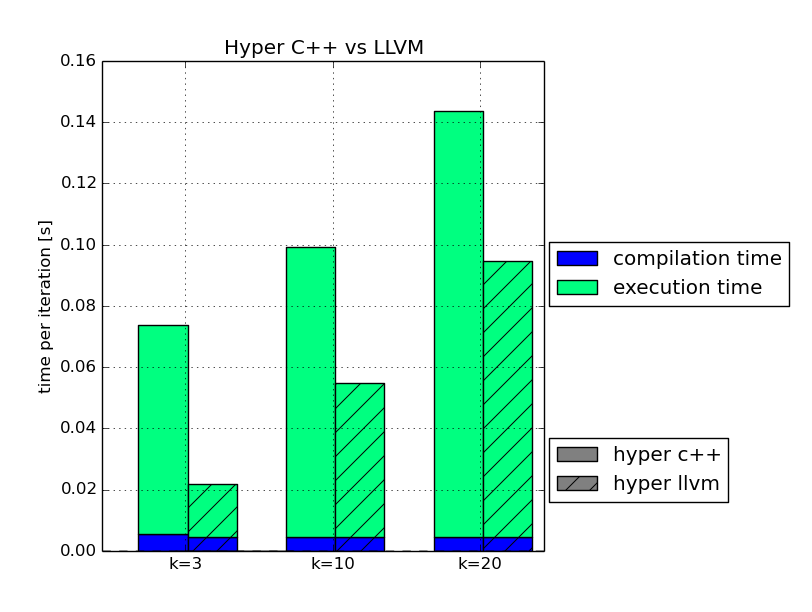
\includegraphics[scale=0.4, trim="0cm 1.5cm 0cm 0cm"]{figures/charts/hyper_network}
  \caption[3D Network - Time per Iteration]{3D Network - Time per Iteration.}
  \label{fig:hyper_network}
\end{figure}


This gives us the first interesting results. First, the compilation time does not differ for between the llvm and c++ version for the network data set. This is interesting since the C++ version is implementing kMeans in C++ using only LLVM functions, while the second version implements everything in LLVM. 
Nevertheless, the main functions remain in LLVM for both implementations. Computing the distance, updating the centers, all those functions are generated LLVM code. In C++ these functions gets generated as functions callable from C++, while in the LLVM version, the code is directly embedded into an LLVM program structure. The difference between the two seems to be insignificant.
How about the execution time? Here, the LLVM version shows a far better time per iteration, actually 4, 2 and 1.5 times faster compared to the C++ version for k equals 3, 10 and 20, respectively. There are two explanations: As already described, the C++ implementation has many function calls between the compile time and the runtime system, while the LLVM version does not. These calls are expensive. why?
The second advantage is that the algorithm is compiled in LLVM code, which produces a very efficient code, optimized on a lower level than C++ code.


\begin{table}[htsb]
  \caption[High Dimensional - Time per Iteration]{High Dimensional - Time per Iteration.}\label{tab:hd_serial}
  \centering
  \begin{tabular}{l l l l l}
    \toprule
      & HyPer C++ & & HyPer LLVM & \\
      k & compilation[s] & execution[s] & compilation[s] & execution[s] \\
    \midrule
      3  & 0.1278 & 0.0522 & 0.0933 & 0.0327 \\
      10 & 0.1287 & 0.1171 & 0.0933 & 0.0706 \\
      20 & 0.1299 & 0.2070 & 0.0933 & 0.1252 \\
    \bottomrule
  \end{tabular}
\end{table}


\begin{figure}[htsb]
  \centering
  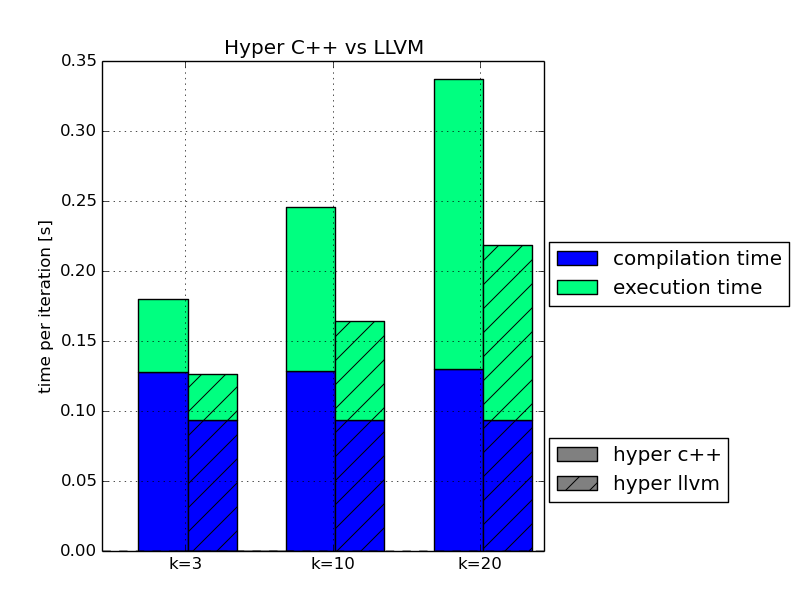
\includegraphics[scale=0.4, trim="0cm 1.5cm 0cm 0cm"]{figures/charts/hyper_50000}
  \caption[High Dimensional - Time per Iteration]{High Dimensional - Time per Iteration.}
  \label{fig:hyper_50000}
\end{figure}



\begin{table}[htsb]
  \caption[Medium Size High Dimensional - Time per Iteration]{Medium Size High Dimensional - Time per Iteration.}
  \label{tab:med_hd_serial}
  \centering
  \begin{tabular}{l l l l l}
    \toprule
      & HyPer C++ & & HyPer LLVM & \\
      k & compilation[s] & execution[s] & compilation[s] & execution[s] \\
    \midrule
      3  & 0.1127 & 16.2787 & 0.0935 & 10.3302 \\
      10 & 0.1127 & 34.0051 & 0.0935 & 22.0209 \\
      20 & 0.1126 & 59.2904 & 0.0935 & 38.7046 \\
    \bottomrule
  \end{tabular}
\end{table}

\begin{figure}[htsb]
  \centering
  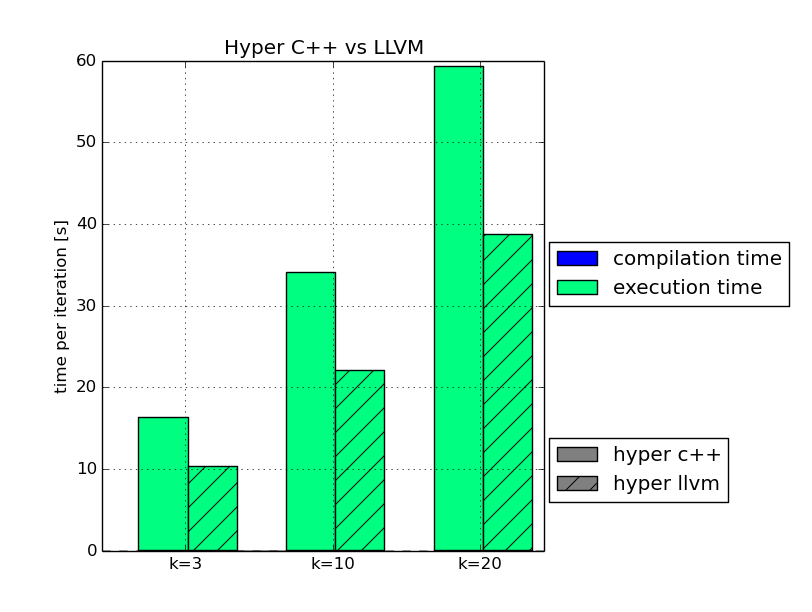
\includegraphics[scale=0.4, trim="0cm 1.5cm 0cm 0cm"]{figures/charts/hyper_15Mxhd}
  \caption[Medium Size High Dimensional - Time per Iteration]{Medium Size High Dimensional - Time per Iteration.}
  \label{fig:hyper_15Mxhd}
\end{figure}



Table: high dim shows the same experiment for the high dimensional data set. This time, the compilation time differs between the c++ and the llvm implementation: The c++ version takes 150% longer. The difference in the running time is similar to the network data set. However, the main difference to the network data set is that the compilation time is actually larger than the execution time for small k, such as k = 3. For k = 10, the compilation and execution times are almost equal, and for k= 20, the execution of kMeans is finally larger than compilation time. 
The increase of compilation time results in the high dimensionality: For each dimension, additional code has to be generated. Therefore, a data set with four dimension is faster to compile than a data set with 50 dimensions.
why compilation time differ?
We also run the C++ and the LLVM implementation on the medium and large data set. The results are shown in table med and table large. The compilation time is very low again, although the number of instances is much higher compared to the high dimensional data set. This proves that the compilation time is dependent on the dimensionality of the data, and not on the data size.


\begin{table}[htsb]
  \caption[Medium Size - Time per Iteration]{Medium Size - Time per Iteration.}
  \label{tab:med_serial}
  \centering
  \begin{tabular}{l l l l l}
    \toprule
      & HyPer C++ & & HyPer LLVM & \\
      k & compilation[s] & execution[s] & compilation[s] & execution[s] \\
    \midrule
      3  & 0.0041 & 2.3779 & 0.0047 & 0.9191 \\
      10 & 0.0041 & 3.2856 & 0.0047 & 2.1001 \\
      20 & 0.0041 & 4.6765 & 0.0047 & 3.4518 \\
    \bottomrule
  \end{tabular}
\end{table}



\begin{table}[htsb]
  \caption[Large Size - Time per Iteration]{Large Size - Time per Iteration.}
  \label{tab:large_serial}
  \centering
  \begin{tabular}{l l l l l}
    \toprule
      & HyPer C++ & & HyPer LLVM & \\
      k & compilation[s] & execution[s] & compilation[s] & execution[s] \\
    \midrule
      3  & 0.0088 & 37.2804 & 0.0097 & 18.3734 \\
      10 & 0.0088 & 62.0034 & 0.0097 & 40.4783 \\
      20 & 0.0191 & 92.5868 & 0.0097 & 67.2364 \\
    \bottomrule
  \end{tabular}
\end{table}


Figure 3 and 4 depict the compilation and execution in a bar chart. Since the compilation time does not depend on the number of instances but on the dimensions, which are low in that example, the compilation time is not even visible. However, execution time increases with the number of instances. As in all the previous experiments as well, execution time of the LLVM implementation is much faster compared to the C++ version. Regarding the large data set, the LLVM version is faster by around 20 seconds per iteration. 

In conclusion, the compilation time is does not grow much if the number of instances gets large but if the number of dimensions grows. Usually, the execution time outnumbers the compilation time by several factors. The only exception is a small, high dimensional data set as shown in the experiment. Here, the compilation can be the bottleneck of the kMeans algorithm.

Another result is that the execution time, growing by number of instances, is much faster for the LLVM implementation since there is almost no communication between C++ and LLVM code. On the other hand, the compilation time is roughly the same. Therefore the LLVM version was always the better choice regarding the running time of the kMeans algorithm.


\section{Performance Test}

In this section we compare HyPer to R and julia’s implementation of kMeans. All programs are executed in serial. As algorithm, the Lloyed algorithm with a maximum iteration number of ten is chosen. Apart from the large data set, the algorithm is executed 100 times for k equals 3, 10 and 20, respectively. For the large data set, the algorithm is only executed ten times. The result is presented as the time per iteration. 

The result of the network data set is presented in Table: network. The median, the 90th and 95th percentile are listed to show the variance of the data. As we already know, the HyPer LLVM implementation outnumbers  the C++ version. Julia is the slowest, while R competes quite well with the LLVM version and is even faster for k equals 10 and 20. Figure 1 shows the results as a boxplot.
However, all tested programs differ in time per iterations in a few hundred milliseconds, therefore the differences are not very significant.



\begin{table}[htsb]
  \caption[3D Network - Time per Iteration]{3D Network - Time per Iteration.}
  \label{tab:network_all}
  \centering
  \begin{tabular}{l l l l l l l l l l l l l}
    \toprule
      & \multicolumn{3}{c}{Julia} & \multicolumn{3}{c}{R} & \multicolumn{3}{c}{HyPer C++} & \multicolumn{3}{c}{HyPer LLVM}  \\
      k & 3 & 10 & 20 & 3 & 10 & 20 & 3 & 10 & 20 & 3 & 10 & 20 \\
    \midrule
      50  & 0.21 & 0.22 & 0.29 & 0.03 & 0.04 & 0.08 & 0.08 & 0.10 & 0.14 & 0.02 & 0.06 & 0.10 \\
      50  & 0.27 & 0.30 & 0.32 & 0.06 & 0.06 & 0.09 & 0.08 & 0.10 & 0.14 & 0.02 & 0.06 & 0.10 \\
      50  & 0.31 & 0.35 & 0.35 & 0.08 & 0.07 & 0.10 & 0.08 & 0.10 & 0.14 & 0.02 & 0.06 & nnnn \\
    \bottomrule
  \end{tabular}
\end{table}
\begin{table}[htsb]
  \caption[3D Network - Time per Iteration]{3D Network - Time per Iteration.}
  \label{tab:network_all}
  \centering
  \begin{tabular}{l l l l l l l l l l l l l}
    \toprule
      & \multicolumn{3}{c}{Julia} & \multicolumn{3}{c}{R} & \multicolumn{3}{c}{HyPer C++} & \multicolumn{3}{c}{HyPer LLVM}  \\
      k & 3 & 10 & 20 & 3 & 10 & 20 & 3 & 10 & 20 & 3 & 10 & 20 \\
    \midrule
      50  & 0.21 & 0.22 & 0.29 & 0.03 & 0.04 & 0.08 & 0.08 & 0.10 & 0.14 & 0.02 & 0.06 & 0.10 \\
      50  & 0.27 & 0.30 & 0.32 & 0.06 & 0.06 & 0.09 & 0.08 & 0.10 & 0.14 & 0.02 & 0.06 & 0.10 \\
      50  & 0.31 & 0.35 & 0.35 & 0.08 & 0.07 & 0.10 & 0.08 & 0.10 & 0.14 & 0.02 & 0.06 & nnnn \\
    \bottomrule
  \end{tabular}
\end{table}



\begin{table}[htsb]
  \caption[3D Network - Time per Iteration]{3D Network - Time per Iteration.}
  \label{tab:network_all}
  \centering
  \begin{tabular}{l l l l l l l l l l l l l}
    \toprule
      & \multicolumn{3}{c}{Julia} & \multicolumn{3}{c}{R} & \multicolumn{3}{c}{HyPer C++} & \multicolumn{3}{c}{HyPer LLVM}  \\
      k & 3 & 10 & 20 & 3 & 10 & 20 & 3 & 10 & 20 & 3 & 10 & 20 \\
    \midrule
      50  & 0.21 & 0.22 & 0.29 & 0.03 & 0.04 & 0.08 & 0.08 & 0.10 & 0.14 & 0.02 & 0.06 & 0.10 \\
      50  & 0.27 & 0.30 & 0.32 & 0.06 & 0.06 & 0.09 & 0.08 & 0.10 & 0.14 & 0.02 & 0.06 & 0.10 \\
      50  & 0.31 & 0.35 & 0.35 & 0.08 & 0.07 & 0.10 & 0.08 & 0.10 & 0.14 & 0.02 & 0.06 & nnnn \\
    \bottomrule
  \end{tabular}
\end{table}



\begin{table}[htsb]
  \caption[3D Network - Time per Iteration]{3D Network - Time per Iteration.}
  \label{tab:network_all}
  \centering
  \begin{tabular}{l l l l l l l l l l l l l}
    \toprule
      & \multicolumn{3}{c}{Julia} & \multicolumn{3}{c}{R} & \multicolumn{3}{c}{HyPer C++} & \multicolumn{3}{c}{HyPer LLVM}  \\
      k & 3 & 10 & 20 & 3 & 10 & 20 & 3 & 10 & 20 & 3 & 10 & 20 \\
    \midrule
      50  & 0.21 & 0.22 & 0.29 & 0.03 & 0.04 & 0.08 & 0.08 & 0.10 & 0.14 & 0.02 & 0.06 & 0.10 \\
      50  & 0.27 & 0.30 & 0.32 & 0.06 & 0.06 & 0.09 & 0.08 & 0.10 & 0.14 & 0.02 & 0.06 & 0.10 \\
      50  & 0.31 & 0.35 & 0.35 & 0.08 & 0.07 & 0.10 & 0.08 & 0.10 & 0.14 & 0.02 & 0.06 & nnnn \\
    \bottomrule
  \end{tabular}
\end{table}



\begin{table}[htsb]
  \caption[3D Network - Time per Iteration]{3D Network - Time per Iteration.}
  \label{tab:network_all}
  \centering
  \begin{tabular}{l l l l l l l l l l l l l}
    \toprule
      & \multicolumn{3}{c}{Julia} & \multicolumn{3}{c}{R} & \multicolumn{3}{c}{HyPer C++} & \multicolumn{3}{c}{HyPer LLVM}  \\
      k & 3 & 10 & 20 & 3 & 10 & 20 & 3 & 10 & 20 & 3 & 10 & 20 \\
    \midrule
      50  & 0.21 & 0.22 & 0.29 & 0.03 & 0.04 & 0.08 & 0.08 & 0.10 & 0.14 & 0.02 & 0.06 & 0.10 \\
      50  & 0.27 & 0.30 & 0.32 & 0.06 & 0.06 & 0.09 & 0.08 & 0.10 & 0.14 & 0.02 & 0.06 & 0.10 \\
      50  & 0.31 & 0.35 & 0.35 & 0.08 & 0.07 & 0.10 & 0.08 & 0.10 & 0.14 & 0.02 & 0.06 & nnnn \\
    \bottomrule
  \end{tabular}
\end{table}


\begin{figure}[htsb]
  \raggedleft
  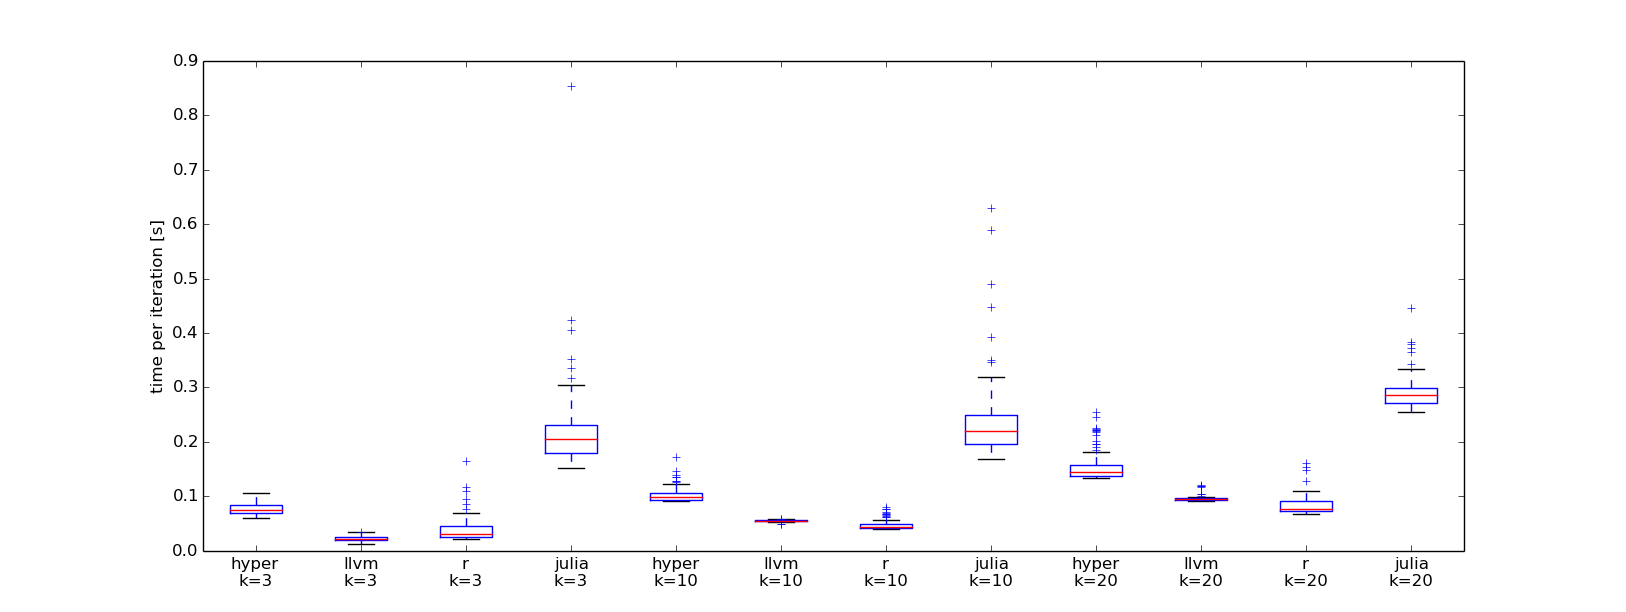
\includegraphics[scale=0.4, trim="0cm 1cm 0cm 0cm"]{figures/charts/network_all}
  \caption[3D Network - Time per Iteration]{3D Network - Time per Iteration.}
  \label{fig:network_all}
\end{figure}

\begin{figure}[htsb]
  \raggedleft
  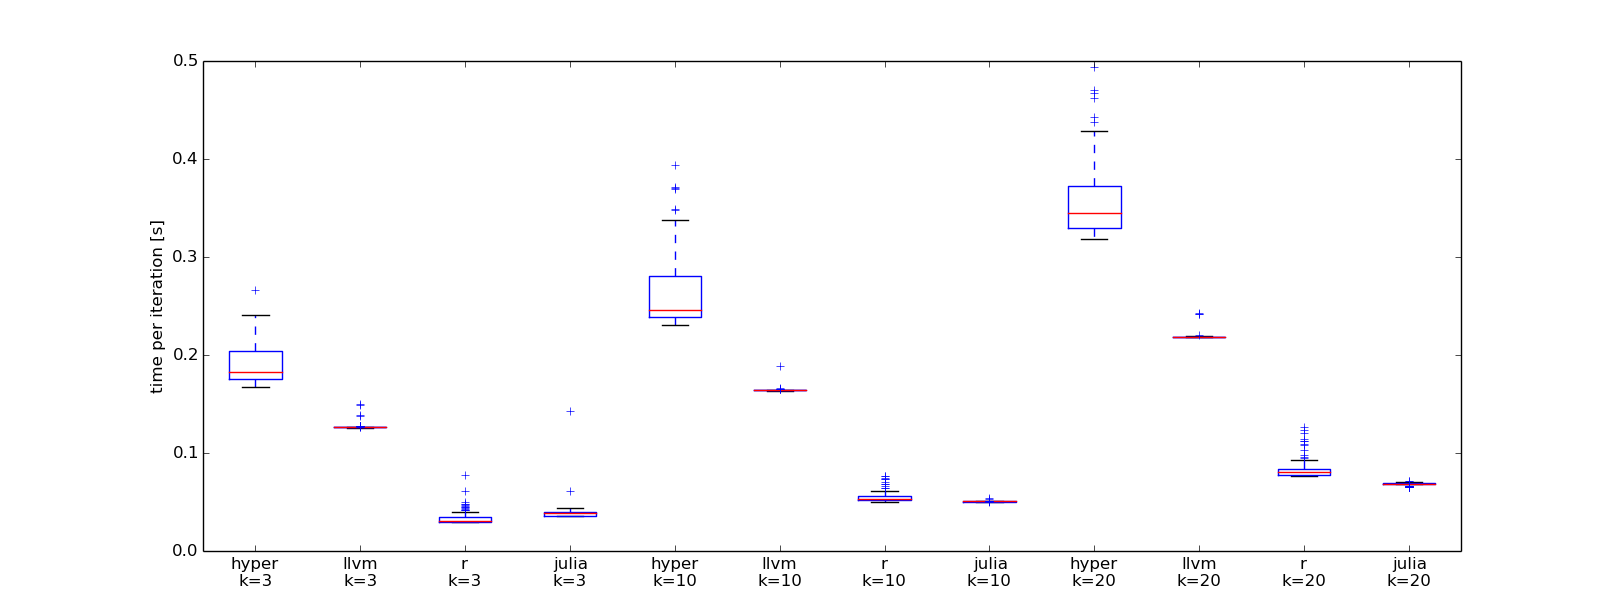
\includegraphics[scale=0.4, trim="0cm 1cm 0cm 0cm"]{figures/charts/50000_all}
  \caption[High Dimensional - Time per Iteration]{High Dimensional - Time per Iteration.}
  \label{fig:50000_all}
\end{figure}

\begin{figure}[htsb]
  \raggedleft
  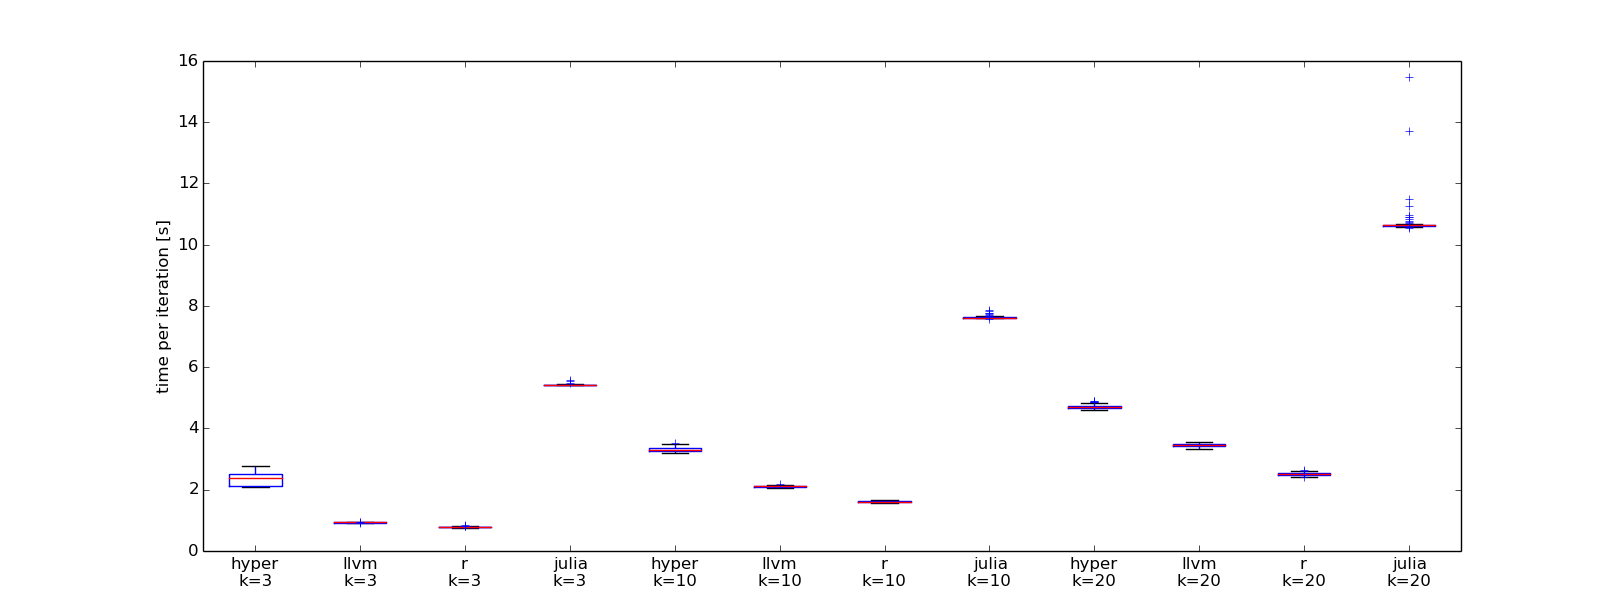
\includegraphics[scale=0.4, trim="0cm 1cm 0cm 0cm"]{figures/charts/15M_all}
  \caption[Medium Size - Time per Iteration]{Medium Size - Time per Iteration.}
  \label{fig:15M_all}
\end{figure}


\begin{figure}[htsb]
  \raggedleft
  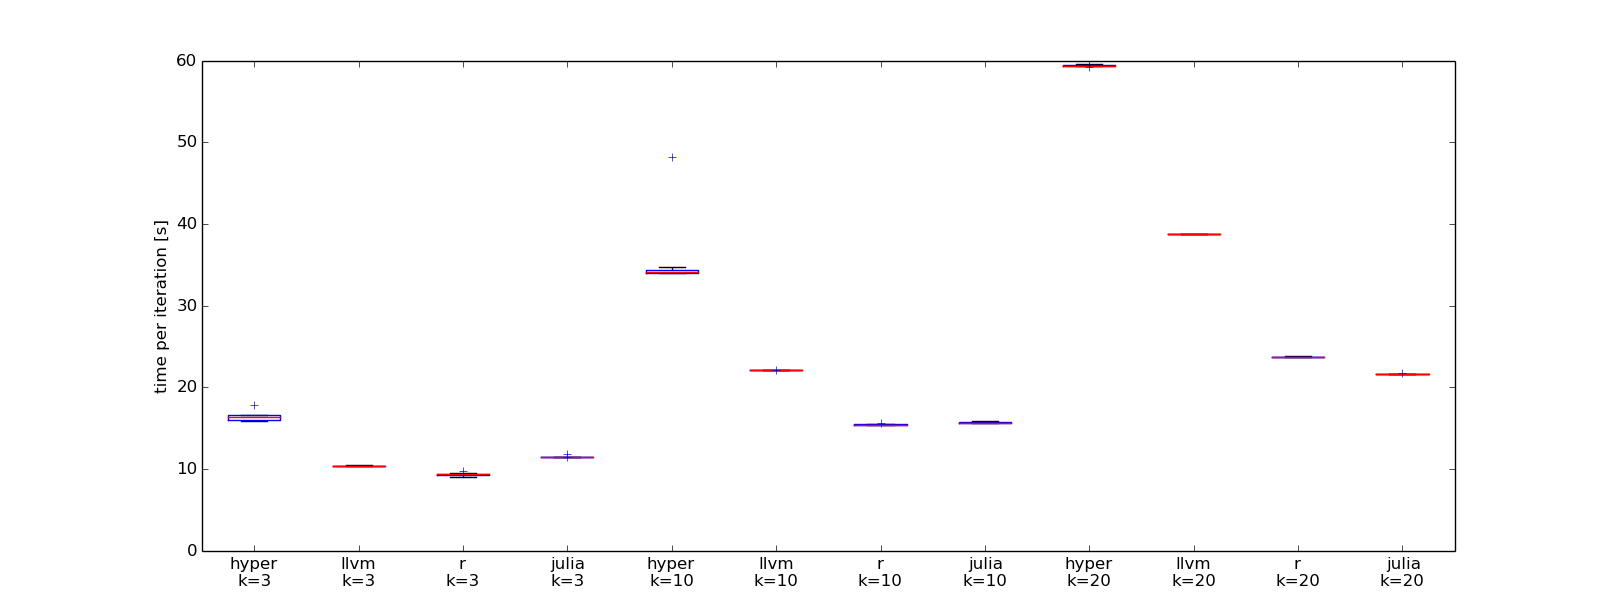
\includegraphics[scale=0.4, trim="0cm 1cm 0cm 0cm"]{figures/charts/15Mxhd_all}
  \caption[Medium Size HD - Time per Iteration]{Medium Size HD - Time per Iteration.}
  \label{fig:15Mxhd_all}
\end{figure}


\begin{figure}[htsb]
  \raggedleft
  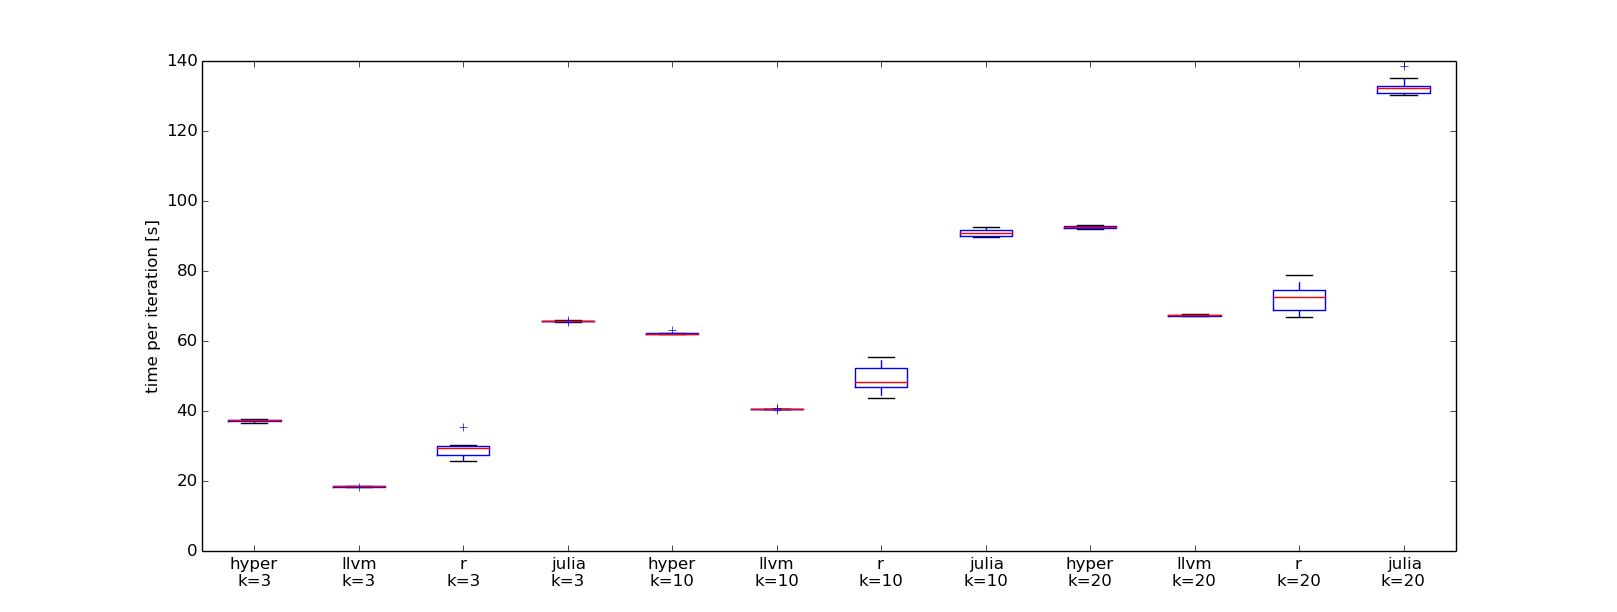
\includegraphics[scale=0.4, trim="0cm 1cm 0cm 0cm"]{figures/charts/150M_all}
  \caption[Large Size - Time per Iteration]{Large Size - Time per Iteration.}
  \label{fig:150M_all}
\end{figure}



\section{Parallel Implementation}


So far we compared the serial execution of the HyPer k-Means operator with julia and R. In 7.4 we figured out that the LLVM implementation outperforms the C++ version on all data sets we tested on. In 7.5 we compared the performance against julia and R and showed that HyPer is able to compete with the existing solutions.
\\
However, as data sets grow serial execution takes more and more time, making real-time data mining almost impossible. To improve performance, HyPer operators benefit from multi-threaded execution. In this section we compare the parallel implementation of the HyPer kMeans operator with the LLVM version and the R implementation. For comparison, we use the medium and the large data set.
\\
Table x depicts the time per iteration for k =3, 10 and 20. As before, the medium, the 90th and 95th percentile of 100 iterations on a 16 core machine are presented. For k equals 3, we see that both the R and the LLVM version are faster than the parallel version. However, with growing k, the parallel version outperforms R and the LLVM version. This is also shown in the bar chart in Figure xx.

\begin{table}[htsb]
  \caption[3D Network - Time per Iteration]{3D Network - Time per Iteration.}
  \label{tab:network_all}
  \centering
  \begin{tabular}{l l l l l l l l l l }
    \toprule
      & \multicolumn{3}{c}{R} & \multicolumn{3}{c}{HyPer C++} & \multicolumn{3}{c}{HyPer LLVM}  \\
      k & 3 & 10 & 20 & 3 & 10 & 20 & 3 & 10 & 20 \\
    \midrule
      50  & 0.03 & 0.04 & 0.08 & 0.08 & 0.10 & 0.14 & 0.02 & 0.06 & 0.10 \\
      90  & 0.06 & 0.06 & 0.09 & 0.08 & 0.10 & 0.14 & 0.02 & 0.06 & 0.10 \\
      95  & 0.08 & 0.07 & 0.10 & 0.08 & 0.10 & 0.14 & 0.02 & 0.06 & nnnn \\
    \bottomrule
  \end{tabular}
\end{table}


The reason for performing better than R and LLVM for growing k is the the running time of the parallel execution is almost independent of k. While R and the LLVM version grow by seconds as k grows, the parallel version grows insignificantly by around 200 milliseconds. 
\\
Unfortunately, for the medium size data set and small k, the parallel version cannot compete with the LLVM and R algorithm.  First, we have to take into account the overhead of the parallel process. Second, we are using the slower C++ version of the HyPer kMeans operator. Even though parts of it are parallelized, we still have all the downsides of many function calls between the runtime and the compile time system and of the high-level C++ constructs.

\begin{figure}[htsb]
  \centering
  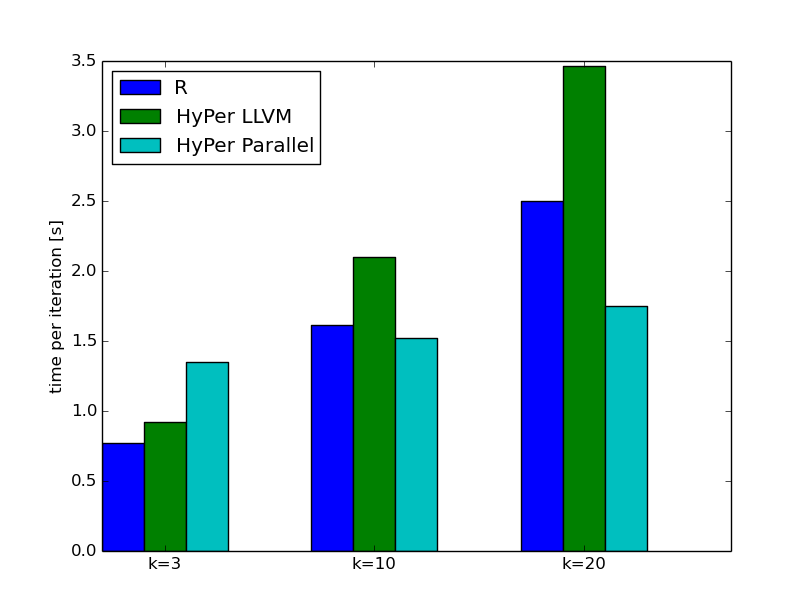
\includegraphics[scale=0.4, trim="0cm 1.5cm 0cm 0cm"]{figures/charts/final_15M}
  \caption[Medium Size - Time per Iteration]{Medium Size - Time per Iteration.}
  \label{fig:final_15M}
\end{figure}

Table x shows the same experiment on the large size data set. The table shows the median, the 90th and the 95th percentile. For better visualization, the bar chart in Figure x depicts the median value of the R, LLVM and parallel execution. 

\begin{table}[htsb]
  \caption[3D Network - Time per Iteration]{3D Network - Time per Iteration.}
  \label{tab:network_all}
  \centering
  \begin{tabular}{l l l l l l l l l l }
    \toprule
      & \multicolumn{3}{c}{R} & \multicolumn{3}{c}{HyPer C++} & \multicolumn{3}{c}{HyPer LLVM}  \\
      k & 3 & 10 & 20 & 3 & 10 & 20 & 3 & 10 & 20 \\
    \midrule
      50  & 0.03 & 0.04 & 0.08 & 0.08 & 0.10 & 0.14 & 0.02 & 0.06 & 0.10 \\
      90  & 0.06 & 0.06 & 0.09 & 0.08 & 0.10 & 0.14 & 0.02 & 0.06 & 0.10 \\
      95  & 0.08 & 0.07 & 0.10 & 0.08 & 0.10 & 0.14 & 0.02 & 0.06 & nnnn \\
    \bottomrule
  \end{tabular}
\end{table}


This time, however, the parallel version outperforms the R and LLVM version for all k’s. Thus, the performance difference gets remarkably as k grows. We experience the same effect as for the medium size data set: A change in k affects only slightly the performance of the parallel version, while it decreases the performance of the serial implementations. 
\\
In the following paragraphs we look at the parallel execution in greater detail. 


\begin{figure}[htsb]
  \centering
  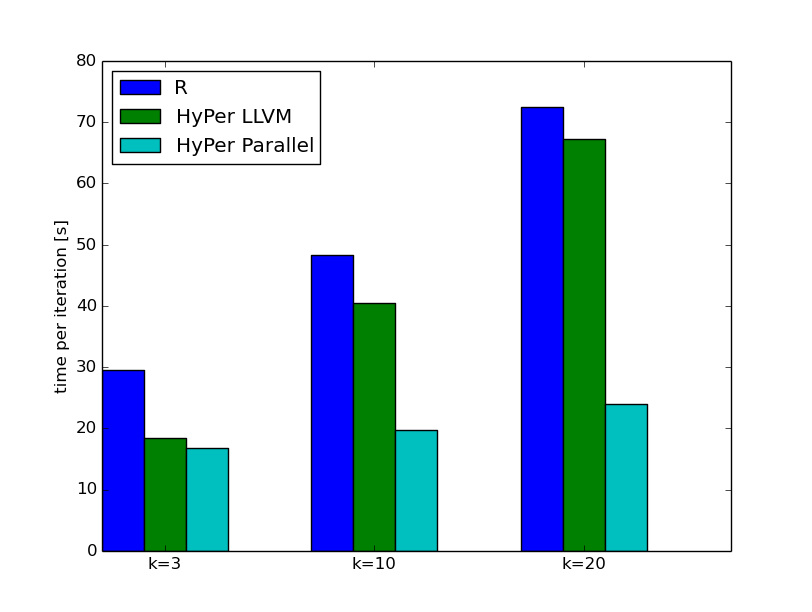
\includegraphics[scale=0.4, trim="0cm 1.5cm 0cm 0cm"]{figures/charts/final_150M}
  \caption[Large Size - Time per Iteration]{Large Size - Time per Iteration.}
  \label{fig:final_150M}
\end{figure}


